\subsection*{LLM в контентно-ориентированных и коллаборативных рекомендациях}
\addcontentsline{toc}{subsection}{LLM в контентно-ориентированных и коллаборативных рекомендациях}

Традиционные рекомендательные системы основываются на двух ключевых подходах – контентно-ориентированном (content-based) и коллаборативном фильтровании. Контентно-ориентированные методы рекомендуют объекты на основании схожести их описаний или характеристик, тогда как коллаборативная фильтрация опирается на информацию о взаимодействиях пользователей (оценки, просмотры и т.п.) для выявления скрытых предпочтений.\footnote{Yandex Handbook: введение в Введение в рекомендательные системы // URL: \url{https://education.yandex.ru/handbook/ml/article/intro-recsys}} Появление больших языковых моделей (LLM) существенно повлияло на оба подхода, позволив усилить их за счёт глубокого анализа текстовых данных и знаний из внешних источников. Ключевое преимущество интеграции LLM в рекомендательные системы – способность извлекать высококачественные семантические представления из текстовых описаний и привносить обширные внешние знания, заложенные в модель в процессе обучения на большом корпусе открытых данных. 
Благодаря этому алгоритмы на основе LLM демонстрируют превосходство в понимании контекста пользовательских запросов, семантики описаний товаров и других текстовых данных в сравнении с классическими подходами. Кроме того, такие модели способны генерировать релевантные рекомендации даже в условиях ограниченного объема данных, эффективно решая проблему «холодного старта» благодаря zero-shot возможностям и способности переносить знания на новые объекты \citep{wu2024surveylargelanguagemodels}.

\textbf{Контентно-ориентированные системы.} Если классические алгоритмы использовали заранее заданные признаки (ключевые слова, категории) или обучения на небольших текстовых моделях, то современные индустриальные решения интегрируют полноценные языковые модели для семантического представления контента. Например, в задаче рекомендаций новостей модели вроде NRMS и Tiny-NewsRec используют предобученные трансформеры для обработки текстов статей. Это позволило лучше справляться со смещением домена (доменные различия в стиле и тематике новостей) и снижать затраты при переносе модели на новые данные, так массивные предобученные модели требуют меньше специфичных для домена данных для адаптации (fine-tuning) или могут лучше обобщать знания на новые, ранее не виданные данные. Таким образом, LLM фактически берут на себя извлечение признаков: так, сервис Amazon Titan Embeddings предлагает готовую модель на основе LLM, превращающую текстовые атрибуты (названия, описания, отзывы) в векторные представления с учётом их смысла \footnote{Amazon Titan Text Embeddings models // URL \url{https://docs.aws.amazon.com/bedrock/latest/userguide/titan-embedding-models.html}} За счёт этого контентно-ориентированные рекомендационные системы стали гораздо точнее выявлять похожие объекты и предпочтения пользователя, что особенно ценно для новых элементов каталога: LLM может сразу «понять» новый товар по описанию и найти ему аналоги, смягчая проблему холодного старта для контентных рекомендаций. Более того, недавние исследования показывают, что модальности-контентные модели (MoRec), использующие передовые языковые энкодеры, уже сравнимы по качеству с традиционными моделями на основе ID (IDRec) даже вне сценариев холодного старта. В работе \citep{yuan2023recommendersystemsidvs} было проведен масштабный эксперимент, резуьтатоми которого является тот факт, что современная контентная модель на базе Transformer-энкодера может не уступать (а иногда и превосходить) чисто коллаборативную модель по точности рекомендаций, даже если оценивать на известных системе элементах.  Таким образом, LLM в сочетании с контентным подходом способны частично заменить коллаборативный фильтр, добывая скрытые связи между элементами через их описания и контекст.

\textbf{Коллаборативные методы}. В классическом коллаборативном фильтровании пользователи и объекты представлены абстрактными ID, и модель учится на матрице взаимодействий. Большие языковые модели предлагают несколько путей усиления таких методов. Во-первых, идентификаторам можно сопоставить текстовую информацию (например, добавить описание пользователя или товара) и позволить языковой модели работать с этой информацией. Такой гибридный подход объединяет преимущества: предобученный языковой энкодер (например, BERT) преобразует описание пользователя или товара в семантический вектор, после чего рекомендации строятся на основе близости этих векторных представлений согласно статье \citep{zhao2024recommendersystemsin}. Во-вторых, можно использовать более фундаментальный подход: полностью формулировать задачу рекомендации как задачу языка. В этом случае история взаимодействий пользователя превращается в текст (например, последовательность просмотренных фильмов), а языковая модель, GPT-подобная, используется для генерации продолжения – то есть для предсказания следующего фильма как следующего слова в предложении.  Исследователи из компании Amazon \citep{zhang2021languagemodelsasrecommendersystemsevaluations} продемонстрировали такой подход, реформулировав задачу рекоммендации сессии в формат маскированного языкового моделирования (cloze-test) с помощью промптов. В экспериментах на датасете кинорекомендаций без какой-либо специфической тренировки (zero-shot) предобученная языковая модель существенно превзошла случайные рекомендации, что подтверждает наличие полезных коллаборативных знаний в её параметрах. Этот результат показывает перспективу данной области: LLM способны выдавать осмысленные рекомендации прямо «из коробки», обобщая знания о популярных сочетаниях контента, приобретённые при предобучении на больших корпусах данных из открытых интернет источников. В то же время, fine-tuning (дообучение) такой модели под конкретный рекомендательный датасет позволил снизить её изначальные лингвистические смещения (например, склонность рекомендовать самые обсуждаемые в текстах объекты), однако существенного и однозначного преимущества над специализированными алгоритмами вроде GRU4Rec достичь пока не удалось. Сей факт подчёркивает, что прямая замена классического коллаборативного фильтра обычный, недообученной LLM-моделью пока имеет ограничения, и для достижения наилучших результатов LLM часто комбинируют с традиционными ID-методами.

Существует ряд работ, где предпринимаются попытки совместить ID-парадигму с языковой. Например, предложено генерировать для каждого объекта особый текстовый код (так называемый Semantic ID) и таким образом представить пользовательские взаимодействия последовательностью таких кодов для подачи в Transformer-модель согласно исследованию \citep{rajput2023recommendersystemsgenerativeretrieval}. Подобные решения позволяют LLM обрабатывать дискретные идентификаторы, однако требуют усложнения пайплайна (обучение дополнительного кодировщика вроде RQ-VAE для генерации семантических кодовых слов и расширение словаря модели). Несмотря на это, направление объединения коллаборативного фильтра и LLM активно развивается – например, в работе CLLM4Rec предложена единая генеративная модель, сочетающая традиционное представление ID с языковым, для улучшения качества рекомендаций на базе графа взаимодействий \citep{zhu2024collaborativelargelanguagemodel}. Таким образом, большие языковые модели нашли применение как и частью коллаборативных систем (вычисляя более содержательные эмбеддинги пользователей/товаров на основе их описаний), так и самостоятельной моделью, решающая задачу рекомендаций через генерацию текста (списка рекомендуемых элементов или объяснений к ним).

\subsection*{Архитектуры крупных языковых моделей в задачах рекомендаций}
\addcontentsline{toc}{subsection}{Архитектуры крупных языковых моделей в задачах рекомендаций}

Современные LLM почти всегда базируются на архитектуре Transformer, однако различаются по структуре (энкодер, декодер или их сочетание) и режиму работы (дискриминативные vs. генеративные). К наиболее известным архитектурам, применяемым в рекомендательных системах, относятся BERT, GPT и T5 – каждая вносит свой определенный вклад в решение задач рекомендации.

\textbf{BERT (Bidirectional Encoder Representations from Transformers)} -  это трансформер-энкодер, обученный на задаче восстановления пропущенных слов (Masked Language Modeling, MLM) и предсказания следующего предложения (Next Sentence Prediction, NSP). Ключевыми функциями потерь для этих задач являются:
\begin{itemize}
    \item Для MLM:
    \[ \mathcal{L}_{MLM}(\theta) = - \sum_{x \in \mathcal{D}} \sum_{i \in M_x} \log p_\theta(x_i | x_{\setminus M_x}) \]
    где \(\mathcal{D}\) – это обучающий корпус, \(x\) – последовательность токенов, \(M_x\) – множество индексов замаскированных токенов в \(x\), \(x_i\) – замаскированный токен, а \(x_{\setminus M_x}\) – незамаскированные токены.
    \item Для NSP:
    \[ \mathcal{L}_{NSP}(\theta) = - \sum_{(s_A, s_B, l) \in \mathcal{D}} \log p_\theta(l | s_A, s_B) \]
    где \(s_A\) и \(s_B\) – это два предложения, а \(l \in \{0, 1\}\) – метка, указывающая, является ли \(s_B\) следующим предложением после \(s_A\).
\end{itemize}
За счёт би-дирекционального внимания BERT учитывает контекст слева и справа от каждого токена, формируя контекстуально богатое представление текста \citep{devlin2019bert}. Примерная архтитектура BERT модели представлена на рисунке \ref{fig:bert_architecture}.

\begin{figure}[H]
    \centering
    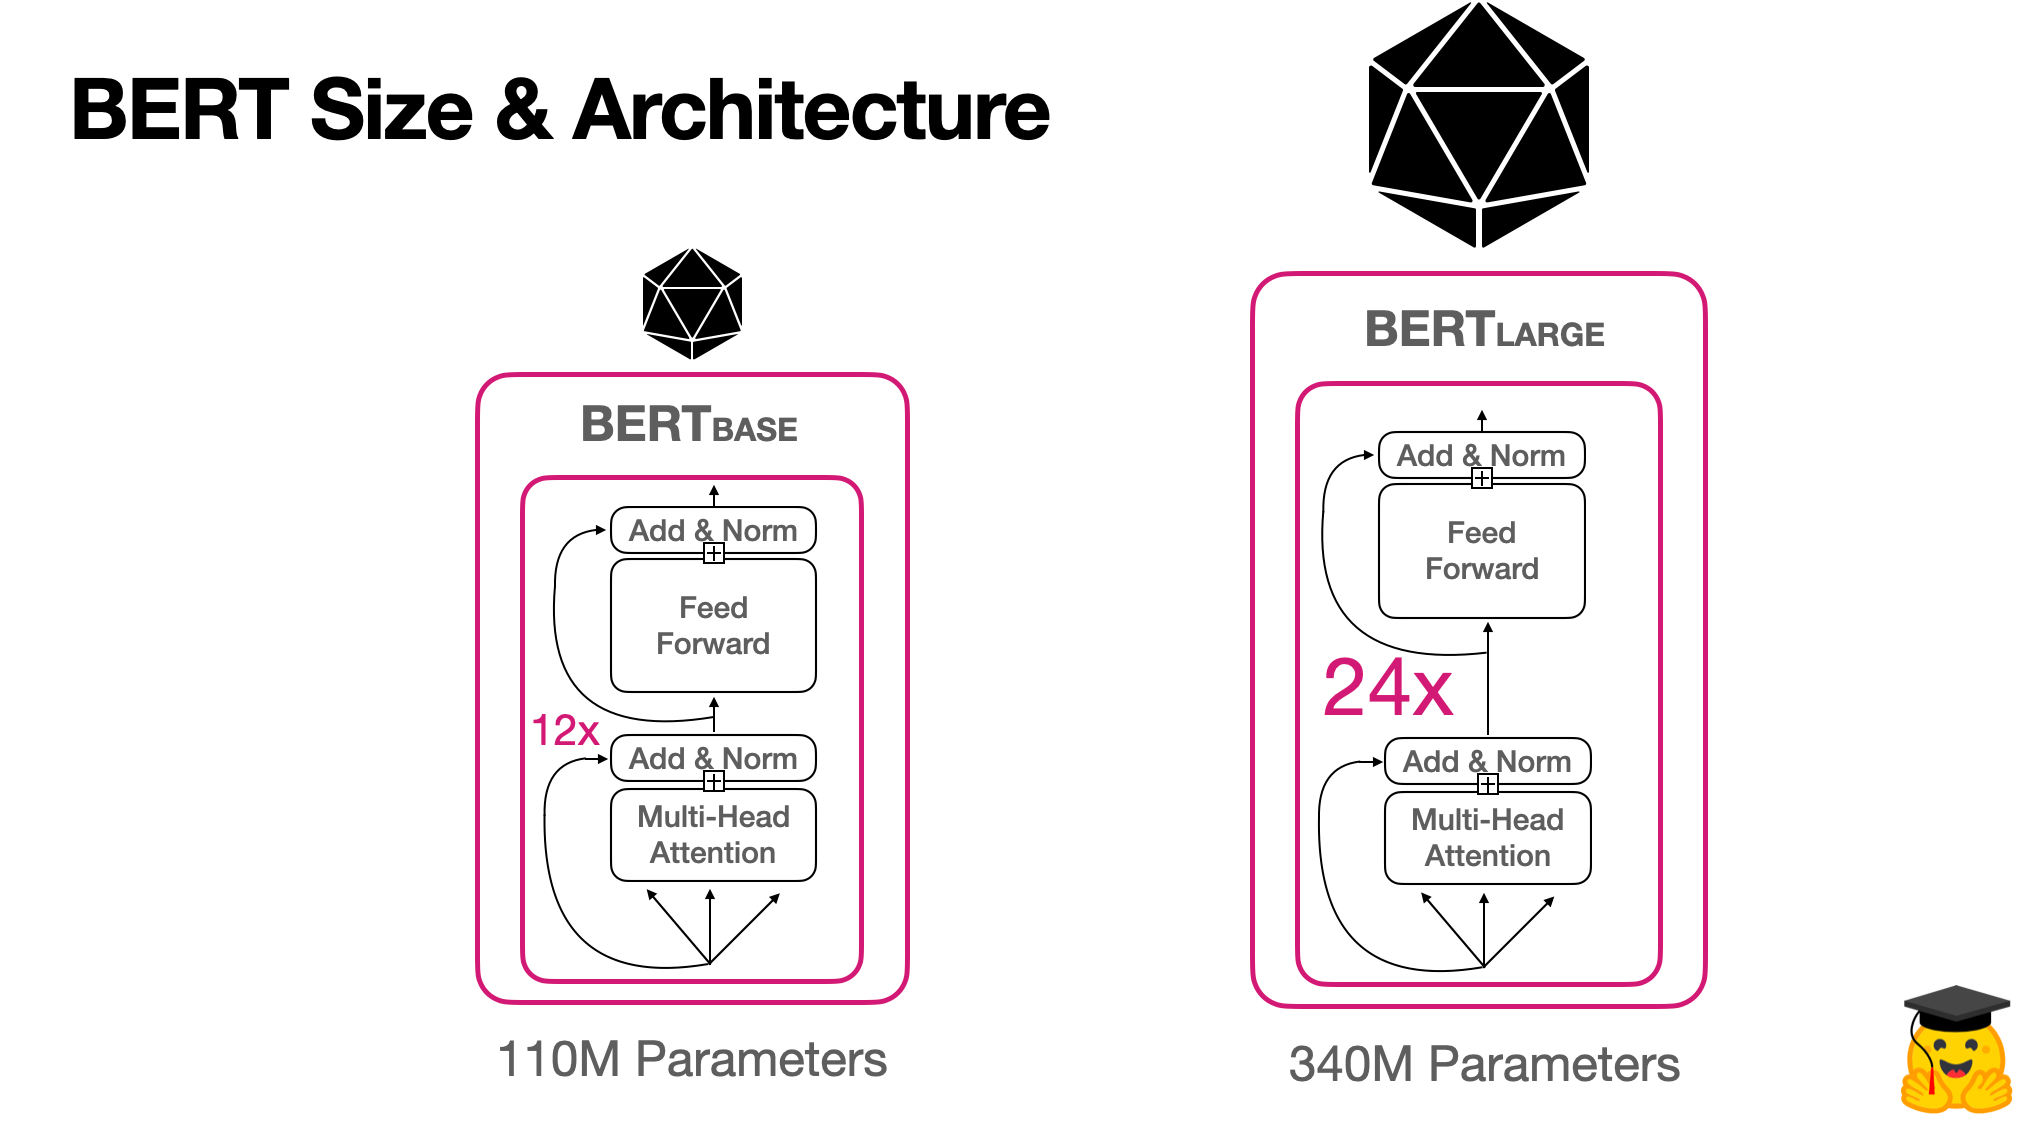
\includegraphics[width=0.8\textwidth]{images/bert.png}
    \caption{Архитектура BERT}
    \label{fig:bert_architecture}
\end{figure}

В рекомендательных системах BERT и его варианты используются главным образом для кодирования контента и учёта последовательности действий. Например, модель BERT4Rec \citep{sun2019bert4rec} адаптировала архитектуру BERT для последовательных рекомендаций: например, история просмотров пользователя можно рассматривать как последовательность «слов», и BERT-энкодер обучался предсказывать пропущенные элементы этой последовательности \footnote{Foundation Model for Personalized Recommendation // URL: \url{https://netflixtechblog.com/foundation-model-for-personalized-recommendation-1a0bd8e02d39}}. Такая модель успешно улавливает сложные паттерны в последовательностях взаимодействий, превзойдя классические методы на откртых датасетах рекомендаций. Кроме того, BERT применяется для извлечения признаков из пользовательских отзывов и описаний товаров – интеграция этих семантических признаков доказала свою пользу в улучшении качества рейтинговых прогнозов


\textbf{GPT (Generative Pre-trained Transformer)} - семейство авторегрессивных моделей-декодеров, генерирующих текст последовательностью слева направо. В отличие от BERT, GPT-модели обучаются предсказывать следующий токен на основе предыдущих, что делает их исключительно мощными в генерации последовательностей и продолжений контекста \citep{zhao2024recommendersystemsin}. Обучение GPT-моделей обычно основано на максимизации правдоподобия следующего токена по всему обучающему корпусу. Функция потерь для авторегрессионного языкового моделирования может быть выражена следующим образом:
\[ \mathcal{L}_{LM}(\theta) = - \sum_{t=1}^{|S|} \log P(w_t | w_1, w_2, \dots, w_{t-1}; \theta) \]
где \(S = (w_1, w_2, \dots, w_{|S|})\) – это последовательность токенов, а \(\theta\) – параметры модели. Модель предсказывает каждый токен \(w_t\), основываясь на предыдущих токенах \((w_1, \dots, w_{t-1})\).
В задачах рекомендации он применяется разными способами. С одной стороны, GPT можно обучить генерировать список рекомендуемых объектов по описанию предпочтений пользователя. Такой подход используется в интерактивных сценариях: например, LLM может по запросу в свободной форме (natural language prompt) последовательно сгенерировать названия треков или фильмов, подходящих под запрос, как будто продолжая диалог с пользователем \citep{palumbo2025text2trackspromptbasedmusicrecommendation}. Однако прямая генерация названий объектов сопряжено с трудностями: модель может ошибаться в названиях, требуется дополнительный шаг сопоставления текста с конкретными ID контента, а длина генерируемых имен замедляет вывод списка. Поэтому в промышленных реализациях генеративный подход видоизменяется – например, модель Text2Tracks (Spotify) предлагает генерировать сразу идентификаторы треков в нужном формате в обход прямой генерации названий. С другой стороны, GPT нашёл применение для диалоговых рекомендательных систем и генерации объяснений. Появление крупной модели ChatGPT показало, что языковой интеллект может вести сложные диалоги, включая сценарий «рекомендательного чат-бота». Исследователи активно эксперементируют с большими языковыми моделями в данной форме, что привело к созданию таких моделей как Chat-REC \citep{gao2023chatrec}, использующую ChatGpt как основу рекомендационного движка. В целом, GPT-архитектуры открыли возможность генеративных рекомендательных систем, где модель буквально пишет рекомендации как ответ на запрос, обогащая опыт пользователя (например, может предложить подборку товаров в форме связного описательного ответа, а не просто списка). 

\textbf{T5 (Text-To-Text Transfer Transformer)} - архитектура энкодер-декодер, разработанная командой Google, в которой любая задача обработки текста представляется в формате «текст на входе – текст на выходе». T5 обучается унифицированно решать разные NLP-задачи, превращая, например, классификацию в задачу порождения слова "positive" или "negative" в ответ на промпт с отзывом, и т.д. Модель обучается с использованием стандартной функции потерь для последовательностей (sequence-to-sequence), такой как перекрестная энтропия, по всему набору разнообразных текстовых задач. Обучающая цель T5 может быть представлена как:
\[ \mathcal{L}_{Seq2Seq}(\theta) = - \sum_{(X, Y) \in \mathcal{D}} \sum_{t=1}^{|Y|} \log p_\theta(y_t | y_{<t}, X) \]
где \(X\) – входная текстовая последовательность (например, задача с инструкцией), \(Y = (y_1, \dots, y_{|Y|})\) – целевая текстовая последовательность, \(\mathcal{D}\) – обучающий набор данных, а \(\theta\) – параметры модели. Модель генерирует каждый токен целевой последовательности \(y_t\), основываясь на предыдущих токенах этой последовательности \(y_{<t}\) и полной входной последовательности \(X\). Такая универсальность оказалась востребованной и в рекомендациях: на базе T5 была создана серия моделей, позволяющих единым образом решать множество рекомендательных задач. Пример – модель P5 (Personalized Prompted PLM), где предобученный T5 взят за основу и дообучен на различных задачах рекомендаций одновременно \citep{geng2022recommendationaslanguageprocessing}. Для этого все данные (матрица взаимодействий, профили пользователей, тексты обзоров, описания товаров) были сконвертированы в текстовые шаблоны-подсказки (prompts). Пользователи и объекты в этих промптах представлены специальными токенами-идентификаторами (например, \texttt{<user\_123>} для пользователя, \texttt{<item\_1>} для объекта), которые добавляются в словарь модели как новые уникальные слова. Модель P5 затем обрабатывает эти текстовые последовательности для генерации требуемого ответа. Например, процесс рекомендации следующего товара для пользователя \texttt{<user\_123>} после взаимодействий с \texttt{<item\_1>} и \texttt{<item\_2>} можно представить так:
\begin{itemize}
    \item \textbf{Входной промпт (Input Prompt):} Текстовая последовательность, кодирующая запрос пользователя и его историю.
    \begin{center}
    \texttt{<user\_123> liked <item\_1>, <item\_2>. Recommends: ?}
    \end{center}
    \item \textbf{Выход модели (Model Output):} Сгенерированный моделью специальный токен, представляющий идентификатор рекомендуемого товара.
    \begin{center}
    \texttt{<item\_42>}
    \end{center}
\end{itemize}
Здесь \texttt{<item\_42>} — это сгенерированный моделью идентификатор рекомендуемого товара. Благодаря этой схеме один и тот же T5 научается выполнять сразу несколько функций: топ-N рекомендацию, предсказание рейтингов, генерацию текстовых рекомендаций и даже объяснений, просто получая разный текстовый промпт на входе. Подход P5 продемонстрировал, что универсальная LLM может заменить множество узкоспециализированных моделей рекомендаций, если грамотно сформулировать их ввод/вывод в виде текста. Помимо P5, появляются и другие крупные модели, адаптированные под рекомендации: например, M6-Rec – мультимодальный трансформер с сотнями миллиардов параметров, применённый для персонализации в e-commerce (Alibaba) \citep{cui2022m6recgenerativepretrainedlanguage}. В целом, архитектуры типа T5 особенно полезны там, где требуется совместить несколько источников данных (текст, рейтинги, профили) и выйти за рамки простого ранжирования – то есть позволяют обобщить разные задачи рекомендации в едином текстовом пространстве.

Помимо вышеперечисленных, в исследовательских работах фигурируют и другие архитектуры и семейства моделей. Например, XLNet (успешно применялся для понимания отзывов), Albert и DistilBERT (облегчённые версии BERT), а в новейших работах используются даже диалоговые модели вроде GPT-4/ Gemini Pro. Однако базовые принципы остаются схожими: рекомендации получают выгоду либо от энкодеров, способных тонко анализировать содержание (BERT, RoBERTa и пр.), либо от генеративных декодеров, способных выдавать последовательности в виде рекомендаций или пояснений (GPT-семейство, LLaMA и др.), либо от их комбинации (T5, FLAN-T5, etc.), объединяющей понимание и генерацию.


\subsection*{Фреймворки и платформы для интеграции LLM в рекомендательные системы}
\addcontentsline{toc}{subsection}{Фреймворки и платформы для интеграции LLM в рекомендательные системы}

Активное развитие методов на стыке NLP и рекомендательных систем привело к появлению специализированных библиотек, облегчающих использование LLM в рекомендациях.

Базовой платформой является библиотека Hugging Face Transformers, предоставляющая предобученные модели (GPT, BERT, T5) и средства для их тонкой настройки на данных рекомендаций. Однако для специфических задач рекомендательных систем требуются дополнительные компоненты.

Специализированным решением стал пакет NVIDIA Merlin Transformers 4Rec для последовательных и сессионных рекомендаций. Библиотека интегрируется с экосистемой HuggingFace и предоставляет готовые модули: позиционные эмбеддинги, механизмы маскирования последовательностей, оптимизированное многоголовое внимание. На её основе созданы улучшенные версии BERT4Rec и SASRec, показавшие state-of-the-art результаты.

Для промышленного применения развиваются облачные платформы. Amazon Bedrock включает модель Titan Embeddings, преобразующую текстовые описания товаров в эмбеддинги для использования в рекомендательных движках реального времени. Это позволяет заменить сложные конвейеры обработки текста единым вызовом LLM-модели.

В исследовательской сфере доступны фреймворки Microsoft Recommenders с реализацией BERT4Rec, библиотека RecBole и LangChain для построения диалоговых рекомендателей через цепочки вызовов LLM. 

\subsection*{Актуальные исследования}
\addcontentsline{toc}{subsection}{Актуальные исследования}
Развитие в области больших языковых моделей неприменно приводит к появлению новых исследований, связанных с их применением в рекомендательных системах. 
Например, исследование "Reason4Rec: Крупные языковые модели для рекомендаций с совещательным согласованием предпочтений пользователя" фокусируется на устранении недостатков поверхностного анализа, характерных для современных рекомендательных систем, построенных на основе больших языковых моделей (RecLLM).
Авторы отмечают, что такие системы часто напрямую предсказывают отклик пользователя, не углубляясь в явный процесс рассуждения о его предпочтениях. Этот подход "быстрого мышления" может приводить к ошибкам в сложных ситуациях, чувствительности к смещениям в данных и трудностям с обобщением \citep{fang2025reason4rec}

В качестве решения предлагается концепция "Совещательной Рекомендации" (Deliberative Recommendation). Суть ее в том, чтобы обучить LLM проходить через явный этап обдумывания и генерации рассуждений о предпочтениях пользователя и характеристиках товара перед тем, как сделать окончательное предсказание. Важным элементом этого подхода является использование 'вербализованной обратной связи пользователя', такой как текстовые отзывы, в качестве обучающих сигналов для формирования процесса рассуждения LLM. Этот фреймворк декомпозирует сложный процесс рассуждения на три последовательных этапа, каждый из которых выполняется специализированным экспертным модулем. Эти эксперты реализованы как отдельные адаптеры QLoRA на одной и той же базовой LLM, что позволяет снизить вычислительные затраты

\begin{figure}[H]
    \centering
    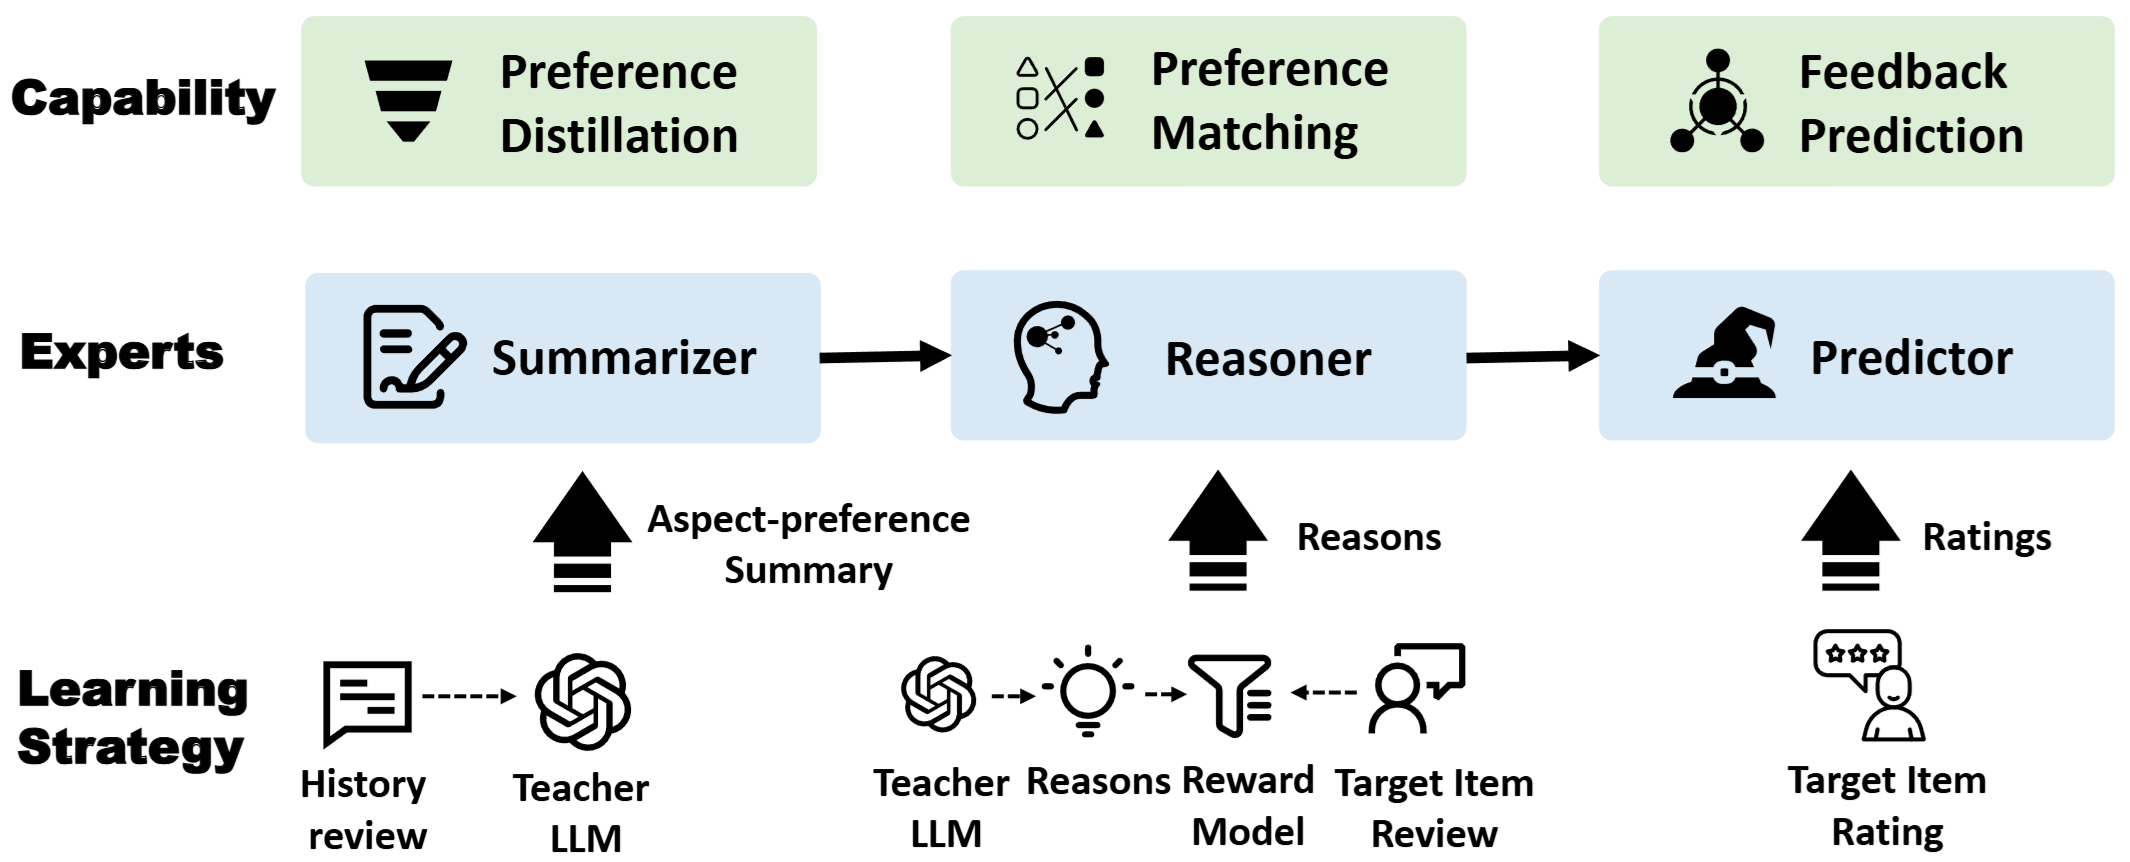
\includegraphics[width=0.8\textwidth]{reason_4_rec.png}
    \caption{Архитектура модели Reason4Rec}
    \label{fig:reason4rec}
\end{figure}

Иной подход к решению проблемы поверхностного анализа можно обнаружить в статье LLMs for User Interest Exploration in Large-scale Recommendation Systems \citep{wang2024llms}. Традиционные рекомендательные системы часто попадают в "ловушку обратной связи". Они учатся на том, что вы делали в прошлом, и рекомендуют похожее. Это мешает открывать для себя что-то совершенно новое и может привести к "усталости от контента".

Данная статья предлагает использовать большие языковые модели (LLM) для того, чтобы помочь пользователям исследовать новые области интересов, выходящие за рамки их привычных предпочтений. Идея в том, чтобы LLM, обладающая обширными знаниями о мире, подсказывала, какие новые направления могут быть интересны пользователю, а уже классическая рекомендательная система подбирала бы конкретные элементы (например, видео, товары) в рамках этих новых направлений.

Авторами предлагается гибридная двухуровневая система:

Верхний уровень (LLM – Стратег):
\begin{itemize}
    \item Вместо того чтобы LLM пыталась предсказать конкретный следующий товар (что сложно и дорого для огромных каталогов), она работает с более крупными "кластерами интересов". Эти кластеры – это группы товаров, объединенных общей темой (например, "Кластер 1: Автобусы, Грузовики, Дороги...", "Кластер 2: Кокос, Банан, Фрукты...").
    \item LLM получает на вход информацию о недавних кластерах интересов пользователя (например, "Недавно я смотрел видео из Кластера 1 и Кластера 2").
    \item Ее задача – сгенерировать описание нового кластера интересов, который мог бы понравиться пользователю, но который отличается от его недавней истории. Например, LLM может предложить: "Новый кластер: Акулы, Подводный мир, Дайвинг...".
    \item Важно, что LLM специально дообучается (fine-tuning) так, чтобы ее текстовые описания новых интересов точно соответствовали одному из заранее определенных кластеров в системе ("контролируемая генерация").
\end{itemize}

Нижний уровень (Классическая рекомендательная система – Тактик):
\begin{itemize}
    \item Получив от LLM описание нового кластера интересов (и его ID), классическая система (например, трансформерная модель последовательных рекомендаций) подбирает уже конкретные товары/видео.
    \item Ключевой момент: поиск товаров ограничивается только теми, которые входят в предложенный LLM новый кластер. Это обеспечивает персонализацию в рамках нового направления.
\end{itemize}

Взяв за основу данное исследование, мы попытались реализовать его на основе данных из открытых источников, а также open-source LLM. 